\documentclass[tikz, border=3pt]{standalone}

\definecolor{rf}{RGB}{230,159,0}
\definecolor{magnet}{RGB}{216, 27, 96}
\definecolor{detector}{RGB}{0,158,115}

\definecolor{lightblue}{RGB}{155,210,220}
\usepackage{circuitikz}
\usepackage{adjustbox}

\usepackage{amsmath}
\DeclareMathOperator{\sgn}{sgn}

%% style for surfaces
\tikzset{surface/.style={draw=gray!70!black, fill=gray!40!white, fill opacity=.6},
  font={\fontsize{20pt}{12}\sffamily}}

\newcommand{\innercolor}{gray!80!black}
\newcommand{\outercolor}{gray!80!white}
\newcommand{\leftcoil}{red!75!gray}
\newcommand{\rightcoil}{green!75!gray}
\pgfmathsetmacro{\coilseparation}{0.02}

\begin{document}

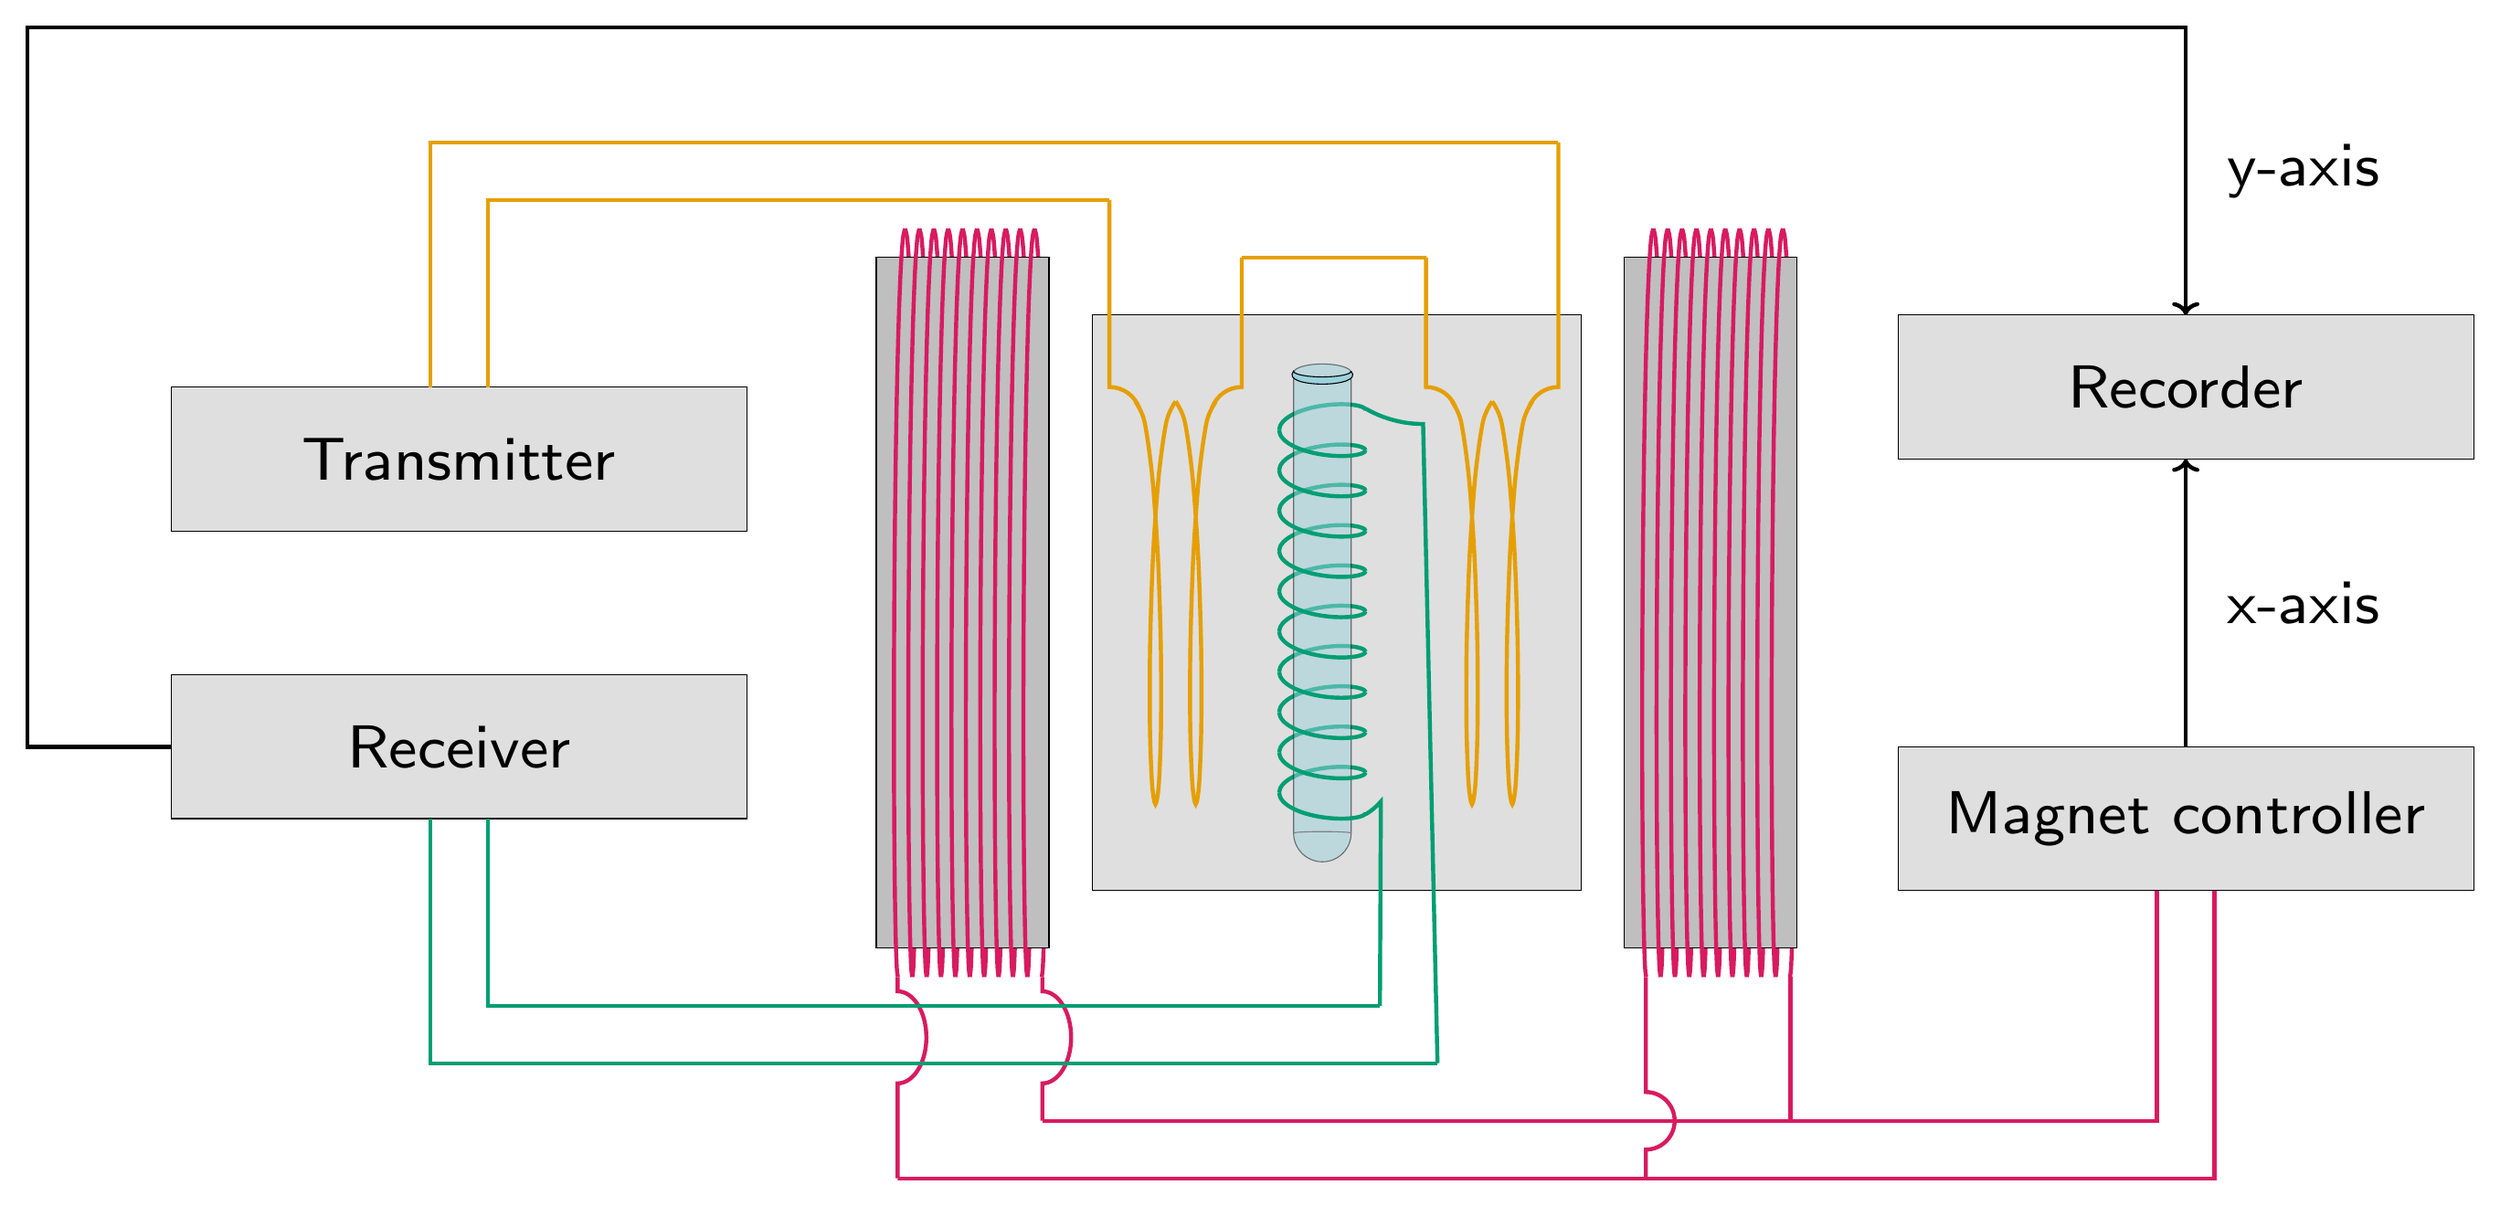
\begin{tikzpicture}[scale = 4, every node/.style={scale=4}]
  \tikzset{
    ultra thin/.style= {line width=0.1pt},
    very thin/.style=  {line width=0.2pt},
    thin/.style=       {line width=0.4pt},% thin is the default
    semithick/.style=  {line width=0.6pt},
    thick/.style=      {line width=0.8pt},
    very thick/.style= {line width=1.2pt},
    ultra thick/.style={line width=1.6pt},
    font={\fontsize{6pt}{12}\sffamily},
    rf/.style={color = rf!100},
    magnet/.style={color = magnet!100},
    detector/.style={color = detector!100},
  }  

    \def\coil#1{
        {0.025 * (2*#1 + \t) + 0.025*sin(\t * pi r))},
        {1.3 * cos(\t * pi r)}
      }

    % left magnet plate
    \begin{scope}[xshift=-10mm]
        \foreach \n in {1,...,10} {
          \draw[magnet, domain={0:1},smooth,variable=\t,samples=15, ultra thick]
          plot (\coil{\n}); 
        }
        \filldraw[fill=gray!50] (-0.05,-1.2) rectangle (0.55,1.2);
        \foreach \n in {0,...,9} {
          \draw[magnet, , domain={1:2},smooth,variable=\t,samples=15, ultra thick]
          plot (\coil{\n});
        }
        \draw[magnet, ultra thick] (0.024, -1.3)  -- (0.024, -1.35) arc (90: -90: 1 mm and 1.6 mm) -- (0.024, -2.0) coordinate (leftplate_left);
        \draw[magnet, ultra thick] (0.527, -1.3)  -- (0.527, -1.35) arc (90: -90: 1 mm and 1.6 mm) -- (0.527, -1.8) coordinate (leftplate_right);
        \end{scope}

        % right magnet plate
      \begin{scope}[xshift=16mm]
        % Draw the part of the coil behind the rectangle
        \foreach \n in {1,...,10} {
          \draw[magnet, domain={0:1},smooth,variable=\t,samples=15, ultra thick]
          plot (\coil{\n}); 
        }
        % Draw the rectangle
        \filldraw[fill=gray!50] (-0.05,-1.2) rectangle (0.55,1.2);

        % Draw the part of the coil in front of the rectangle
        \foreach \n in {0,...,9} {
          \draw[magnet, domain={1:2},smooth,variable=\t,samples=15, ultra thick]
          plot (\coil{\n});
        }
        \draw[magnet, ultra thick] (0.024, -1.3)  -- (0.024, -1.70) arc (90: -90: 1 mm and 1 mm) -- (0.024, -2.0) coordinate (rightplate_left);
        \draw[magnet, ultra thick] (0.527, -1.3) -- (0.527, -1.8) coordinate (rightplate_right);
      \end{scope}


      \def\narrowcoil#1{
        {0.07* (2*#1 + \t) + 0.05*sin(\t * pi r)) - 0.8},
        {0.15 * cos(\t * pi r) - 0.4}
      }
      
      \begin{scope}[xshift=0.5cm]
        % Gray box
        \filldraw[fill=gray!25] (-0.8,-1.0) rectangle (0.9,1.0);
      \end{scope}

      % Test tube
      \begin{scope}[xshift=0.1cm]
         \foreach \n in {1,...,10} {
          \draw[detector, domain={0:1},smooth,variable=\t,samples=15, rotate=90, ultra thick] 
          plot (\narrowcoil{\n}); 
        }

        \draw[fill=lightblue, opacity=.5] (0.3, 0.8) -- (0.3, -0.8)  arc (180:360:1 mm and 1mm)
        -- (0.5, 0.8) arc (0:360: 1mm and 0.3 mm); 
        \draw[fill=lightblue] (0.5, 0.805) to[out=-50,in=230, looseness=1] (0.3,0.805) arc (180:360:1mm and 0.2mm);
        \draw[gray] (0.5,-0.8) arc(0:180:1mm and 0.05mm);
        
        \foreach \n in {0,...,9} {
          \draw[detector, domain={1:2},smooth,variable=\t,samples=15, rotate=90, ultra thick]
          plot (\narrowcoil{\n});
        }

        \draw [detector, ultra thick] (0.55, -0.735) arc(-60:-40:2mm)  -- (0.6,-1.4) coordinate (tube_left);
        \draw [detector, ultra thick] (0.55, 0.675) arc(-120:-90:4mm) -- (0.8,-1.6) coordinate (tube_right);
      \end{scope}

      \def\widecoil#1{
        {0.07* (2*#1 + \t) + 0.05*sin(\t * pi r)) - 0.8},
        {0.7 * cos(\t * pi r) - 0}
      }

      % Left RF
      \begin{scope}[xshift=0.65cm]
        \foreach \n in {0,...,1} {
          \draw[rf, domain={0:2},smooth,variable=\t,samples=15, ultra thick]
          plot (\widecoil{\n});
        }
        \draw[rf, ultra thick] (-0.43, 1.2)  coordinate (rfleft_right) -- (-0.43, 0.75) arc (90: 160: 0.11);
        \draw[rf, ultra thick] (-0.89, 1.4)  coordinate (rfleft_left) -- (-0.89, 0.75) arc (90: 20: 0.11);
      \end{scope}

      % Right RF
      \begin{scope}[xshift=1.75cm]
        \foreach \n in {0,...,1} {
          \draw[rf, domain={0:2},smooth,variable=\t,samples=15, ultra thick]
          plot (\widecoil{\n});
        }
        \draw[rf, ultra thick] (-0.43, 1.6)  coordinate (rfright_right) -- (-0.43, 0.75) arc (90: 160: 0.11);
        \draw[rf, ultra thick] (-0.89, 1.2)  coordinate (rfright_left) -- (-0.89, 0.75) arc (90: 20: 0.11);

        \draw [rf, ultra thick] (rfleft_right) -- (rfright_left) ;
      \end{scope}
      
      \filldraw[fill=gray!25] (-3.5, 0.25) rectangle (-1.5, 0.75)  node[pos=.5] {Transmitter};
      \filldraw[fill=gray!25] (-3.5,-0.75) rectangle (-1.5, -0.25)  node[pos=.5] {Receiver};;
      \draw [rf, ultra thick] (rfright_right) -- (-2.6, 1.6) -- (-2.6, 0.75) ;
      \draw [rf, ultra thick] (rfleft_left) -- (-2.4, 1.4) -- (-2.4, 0.75);

      \draw [detector, ultra thick] (tube_left) -- (-2.4, -1.4) -- (-2.4, -0.75);
      \draw [detector, ultra thick] (tube_right) -- (-2.6,  -1.6) -- (-2.6, -0.75);

      \draw [magnet, ultra thick] (rightplate_right) -- (leftplate_right) -- (3.4,  -1.8) -- (3.4, -1) ;
      \draw [magnet, ultra thick] (rightplate_left) -- (leftplate_left) -- (3.6,  -2.0) -- (3.6, -1);
      \filldraw[fill=gray!25] (2.5, -1.00) rectangle (4.5, -0.5)  node[pos=.5] {Magnet controller};

      \draw [->, ultra thick] (3.5, -0.5) -- (3.5, 0.5) node [midway, right] (TextNode) {x-axis};
      \draw [->, ultra thick] (-3.5, -0.5) -- (-4, -0.5) -- (-4, 2) -- (3.5, 2) -- (3.5, 1.0) node [midway, right] (TextNode) {y-axis};

      \filldraw[fill=gray!25] (2.5, 0.5) rectangle (4.5, 1.0)  node[pos=.5] {Recorder};      
      
  \end{tikzpicture}
\end{document}
